\documentclass[12pt]{article}

\usepackage{graphicx}
\usepackage{amsmath}
\usepackage{amssymb}
\usepackage{natbib}
\usepackage{amsfonts}
\usepackage{multicol}
\usepackage{float}
\usepackage{oldgerm}
\usepackage{bm}
\usepackage{mathtools}
\usepackage{wrapfig}
\usepackage{fancyhdr}
\usepackage[export]{adjustbox}
\usepackage{xcolor}

\pagestyle{empty}

\newcommand{\Avec}{\mathbf A}
\newcommand{\Bvec}{\mathbf B}
\newcommand{\Dvec}{\mathbf D}
\newcommand{\Evec}{\mathbf E}
\newcommand{\Fvec}{\mathbf F}
\newcommand{\Jvec}{\mathbf J}
\newcommand{\Lvec}{\mathbf L}
\newcommand{\Mvec}{\mathbf M}
\newcommand{\Pvec}{\mathbf P}
\newcommand{\Rvec}{\mathbf R}
\newcommand{\Svec}{\mathbf S}
\newcommand{\Tvec}{\mathbf T}
\newcommand{\avec}{\mathbf a}
\newcommand{\bvec}{\mathbf b}
\newcommand{\dvec}{\mathbf d}
\newcommand{\evec}{\mathbf e}
\newcommand{\fvec}{\mathbf f}
\newcommand{\jvec}{\mathbf j}
\newcommand{\kvec}{\mathbf k}
\newcommand{\nvec}{\mathbf n}
\newcommand{\pvec}{\mathbf p}
\newcommand{\rvec}{\mathbf r}
\newcommand{\svec}{\mathbf s}
\newcommand{\vvec}{\mathbf v}
\newcommand{\xvec}{\mathbf x}
\newcommand{\yvec}{\mathbf y}
\newcommand{\zvec}{\mathbf z}
\newcommand{\nablav}{\boldsymbol{\nabla}}
\newcommand{\nablavector}{\vec \nabla}
\newcommand{\alphavec}{\boldsymbol{\alpha}}
\newcommand{\phivec}{\boldsymbol{\phi}}
\newcommand{\thetavec}{\boldsymbol{\theta}}
\newcommand{\omegavec}{\boldsymbol{\omega}}
\newcommand{\tauvec}{\boldsymbol{\tau}}
\newcommand{\epvec}{\boldsymbol{\epsilon}}
\newcommand{\ezero}{\epsilon_{0}}
\newcommand{\mzero}{\mu_{0}}
\newcommand{\unitx}{\mathbf{\hat{x}}}
\newcommand{\unity}{\mathbf{\hat{y}}}
\newcommand{\unitz}{\mathbf{\hat{z}}}
\newcommand{\mubold}{\boldsymbol{\mu}}
\newcommand{\uniti}{\hat{\boldsymbol{\imath}}}
\newcommand{\unitj}{\hat{\boldsymbol{\jmath}}}
\newcommand{\unitk}{\hat{\boldsymbol{\mathit{k}}}}
\newcommand{\unitn}{\hat{\mathbf n}}
\newcommand{\unitr}{\hat{\mathbf r}}
\newcommand{\unitphi}{\hat{\boldsymbol{\phi}}}
\newcommand{\unittheta}{\hat{\boldsymbol{\theta}}}

\newcommand{\bit}{\begin{itemize}}
\newcommand{\eit}{\end{itemize}}

\setlength{\headsep}{0.5cm}
\setlength{\oddsidemargin}{-0.5cm}
\setlength{\textwidth}{16.5cm}
\setlength{\textheight}{24cm}
\voffset = -2cm

\pagestyle{fancy}
\fancyhf{}
\rfoot{
\includegraphics[width=1.0in]{cnm.png}}
\lfoot{Homework 4}
\begin{document}

%{\bf \underline{STUDENT NAME}:} 
%\vspace{1cm}

\begin{center}
%\date{10/02/18-10/09/18}
\hfil
{\large\bf {ENGR 2910-101: Circuit Analysis}}
\hfill Instructor: Leo Silbert \\
Homework 4: 09/21/21 \hfill Due: 09/28/21\\
\hrulefill\\
\end{center}

%{\em Show all your working to ensure you obtain full points. Partial
%  credit will be given for correct algebraic steps if you fail to
%  obtain the correct final answer.}\\

%\newpage


\noindent
{\bf Question 1} [10] %P2-18

\begin{figure}[h!]
  \centering 
 \vspace{-0.1in}
 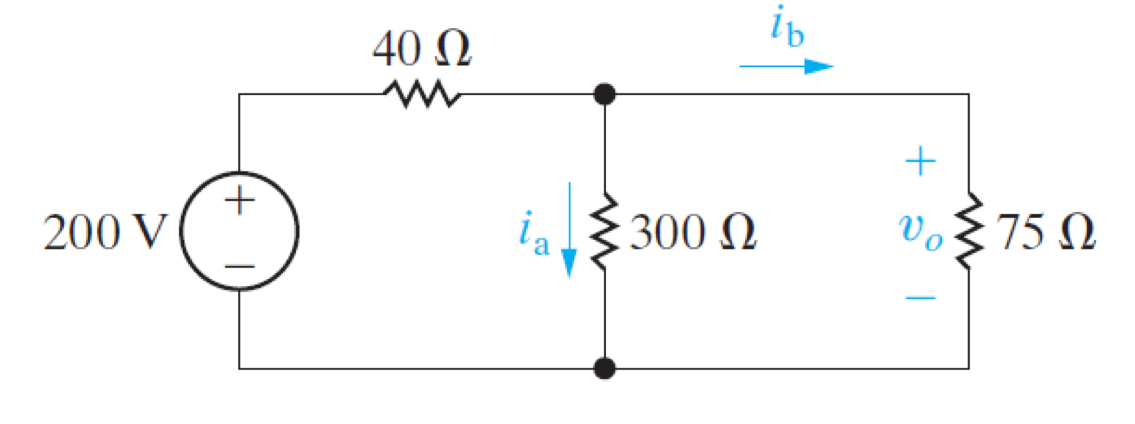
\includegraphics[clip,width=0.7\textwidth]{Fig2-18.png}
\vspace{-0.1in}
\end{figure}
For the circuit shown, find: 

\bit

\item[(a)]

the value of $i_{\text{a}}$,

\item[(b)]

the value of $i_{\text{b}}$,

\item[(c)]

the value of $v_{o}$,

\item[(d)]

the power dissipated in each resistor,

\item[(e)]

the power delivered by the 200 V source.

\eit


\vspace{0.1in}
\noindent
{\bf Question 2} [10] %P2-22

In the circuit below, the current $i_{o} = 2$A.  
\begin{figure}[h!]
     \centering
\vspace{-0.1in}
     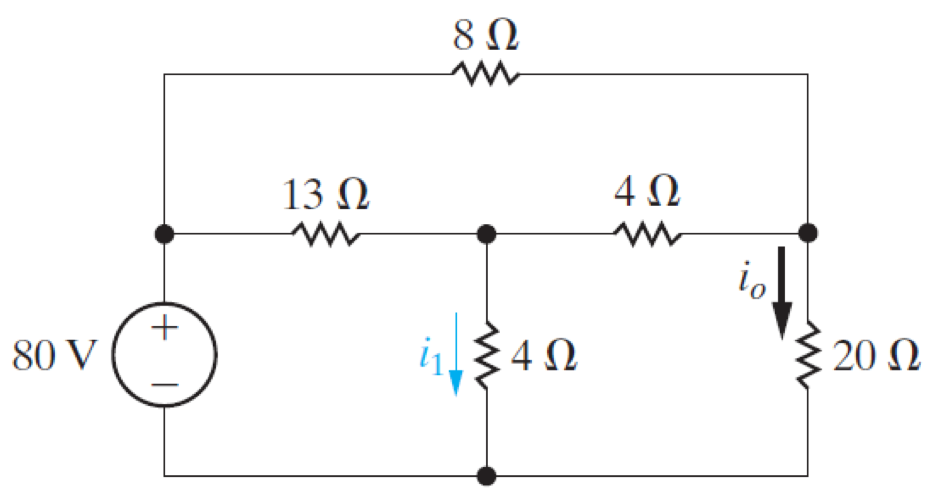
\includegraphics[clip,width=0.6\textwidth]{Fig2-22.png}
\vspace{-0.15in}
\end{figure}
 \bit
\item[(a)]
Find $i_{1}$. 

\item[(b)]
Find the power dissipated in each resistor.

\item[(c)]
Verify that the total power dissipated in the circuit equals the power provided by the voltage source.

\eit

\newpage
\noindent
{\bf Question 3} [10] %P2-27

The variable resistor $R$ is adjusted until $i_{o} = 10$ mA. Find the value of $R$.
\begin{figure}[!h]
  \centering 
  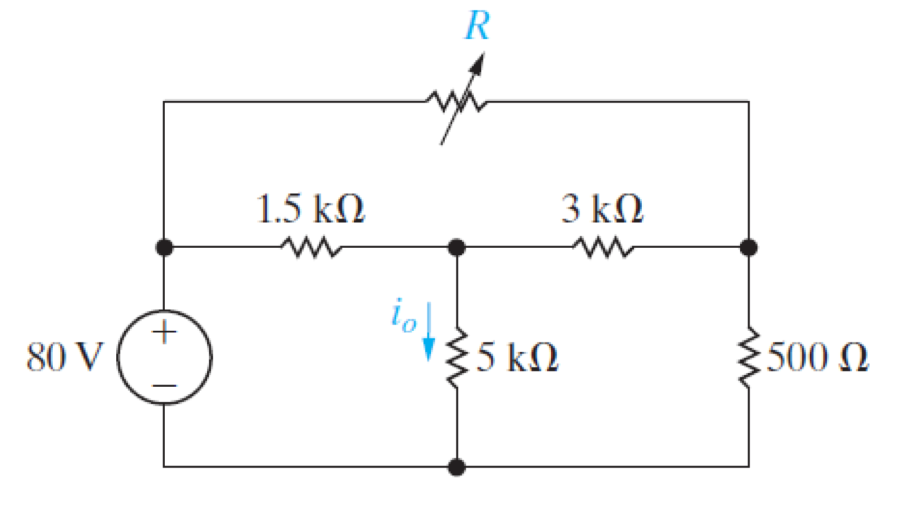
\includegraphics[clip,width=0.6\textwidth]{Fig2-27.png}
\end{figure}

\vspace{0.1in}
\noindent
{\bf Question 4} [10] %P2-29

The voltage and current were measured at the terminals of the device shown.
\begin{figure}[h!]
  \centering 
  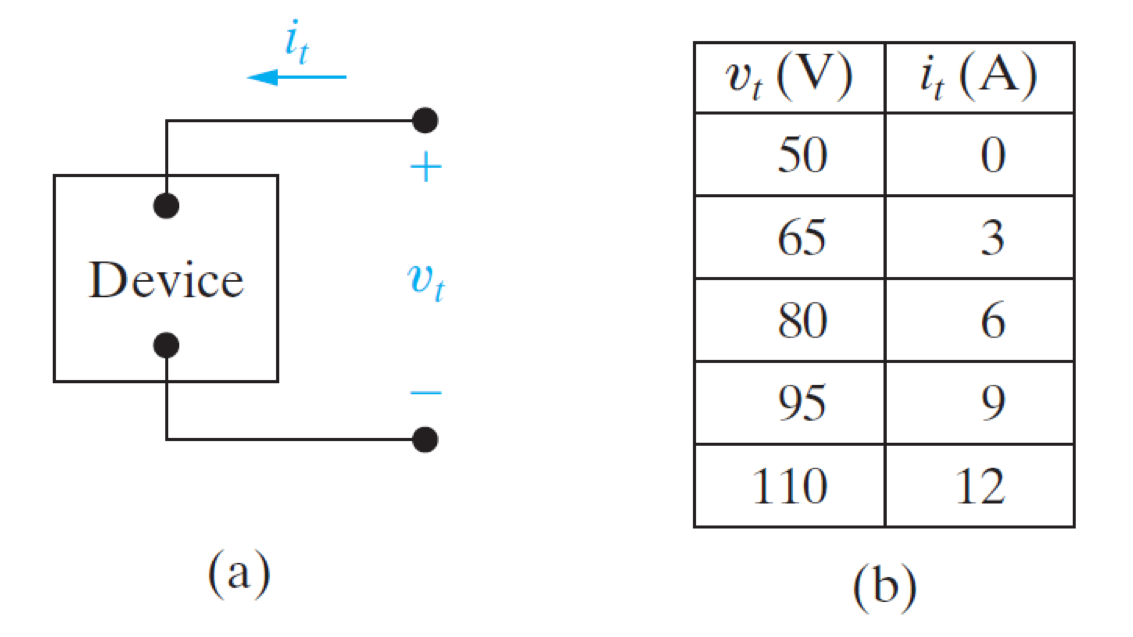
\includegraphics[clip,width=0.5\textwidth]{Fig2-29.png}
\end{figure}
\bit

\item[(a)]

Construct a circuit model for this device using an ideal current source in parallel with a resistor by plotting the data.

\item[(b)]

Use the model to predict the amount of power the device will deliver to a $20 \Omega$ resistor.

\eit

\vspace{0.1in}
\noindent
{\bf Question 5} [10] %P2-34

Find $v_{o}$ and the total power supplied in the circuit.
\begin{figure}[h!]
\centering 
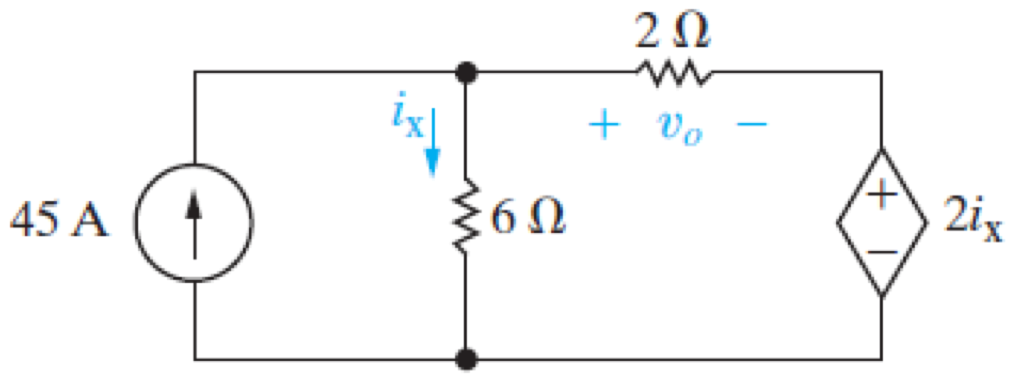
\includegraphics[clip,width=0.6\textwidth]{Fig2-34.png}
\end{figure}
 

\end{document}
